\section{Hierarchy description}

\subsection{Model}

The software's logic is based upon VideoFile base class, from which other classes inherit general infos and features. Specializations of the VideoFile class are Movie, Anime, TvSerie and Match classes. There is only one level of inheritance as shown on the schema below: \\

\begin{center}
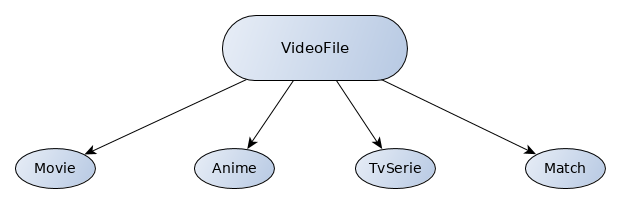
\includegraphics[scale=0.65]{Img/Hierarchy.png}
\captionof{figure}{Types hierarchy schema.}
\end{center}

\begin{itemize}
\item \textbf{VideoFile class:} is the base class of the hierarchy. It represents generic video files such as \emph{amateurs holiday's film} and is characterized by a \emph{title, a genre, a nation} and \emph{a publishing year}.
\item \textbf{Movie class:} child of VideoFile class, represents cinematographic movies and is characterized by every detail of a generic video file plus a \emph{director} and a \emph{length} expressed in minutes.
\item \textbf{Anime class:} child of VideoFile class, represents Japanese animation series and is characterized by the \emph{number of episodes} and the fact that it is still ongoing  or not.
\item \textbf{TvSerie class:} child of VideoFile class, represents tv series characterized by \emph{number of seasons} and the fact that is still ongoing or not.
\item \textbf{SportMatch class:} child of VideoFile class, represents a recording of a sport match, characterized by a belonging \emph{championship}, a \emph{home team} and a \emph{guest team}.
\end{itemize}

\subsection{View}

The GUI has been made with maximum component-reuse in mind. In fact every custom widget, a part from MainWindow, is a refinement and a specialization of another one. Examples are the widget needed to insert an object on Qontainer, that is most part like the one to modify an object; also the insertion and find ones share most of the widgets, preventing exceeding code duplication.

